% ! TeX root = ../../master-thesis.tex

\chapter{Design}
\label{chapter:design}

This chapter presents the abstract solution designed for achieving the
objectives of this project. First, Section \ref{section:design:simulation}
introduces an extension of the base reactive execution model of FRASP with
increased observability and controllability. Then, Section
\ref{section:design:step-simulation} provides a solution to the halting problem
of FRASP simulations. Afterward, Section
\ref{section:design:convergence-simulation} explains the process of performing
aggregate convergence tests leveraging the new simulation models. Finally,
Section \ref{section:design:concurrent-simulation} describes the parallelism
constraints on concurrent simulations.

% ! TeX root = ../../master-thesis.tex

\section{Simulation}
\label{section:design:simulation}

The proposed approach for improving the observability and controllability of
the current simulator is to provide an interface on top of the base reactive
execution model of FRASP (Figure \ref{figure:simulation}). The design of this
interface abstracts from the underlying \ac{FRP} framework, specifically
Sodium, and from the approach adopted for managing the propagation of change in
the computational graph (e.g., concrete implementations may support
concurrency).

\begin{figure}[!ht]
  \centering
  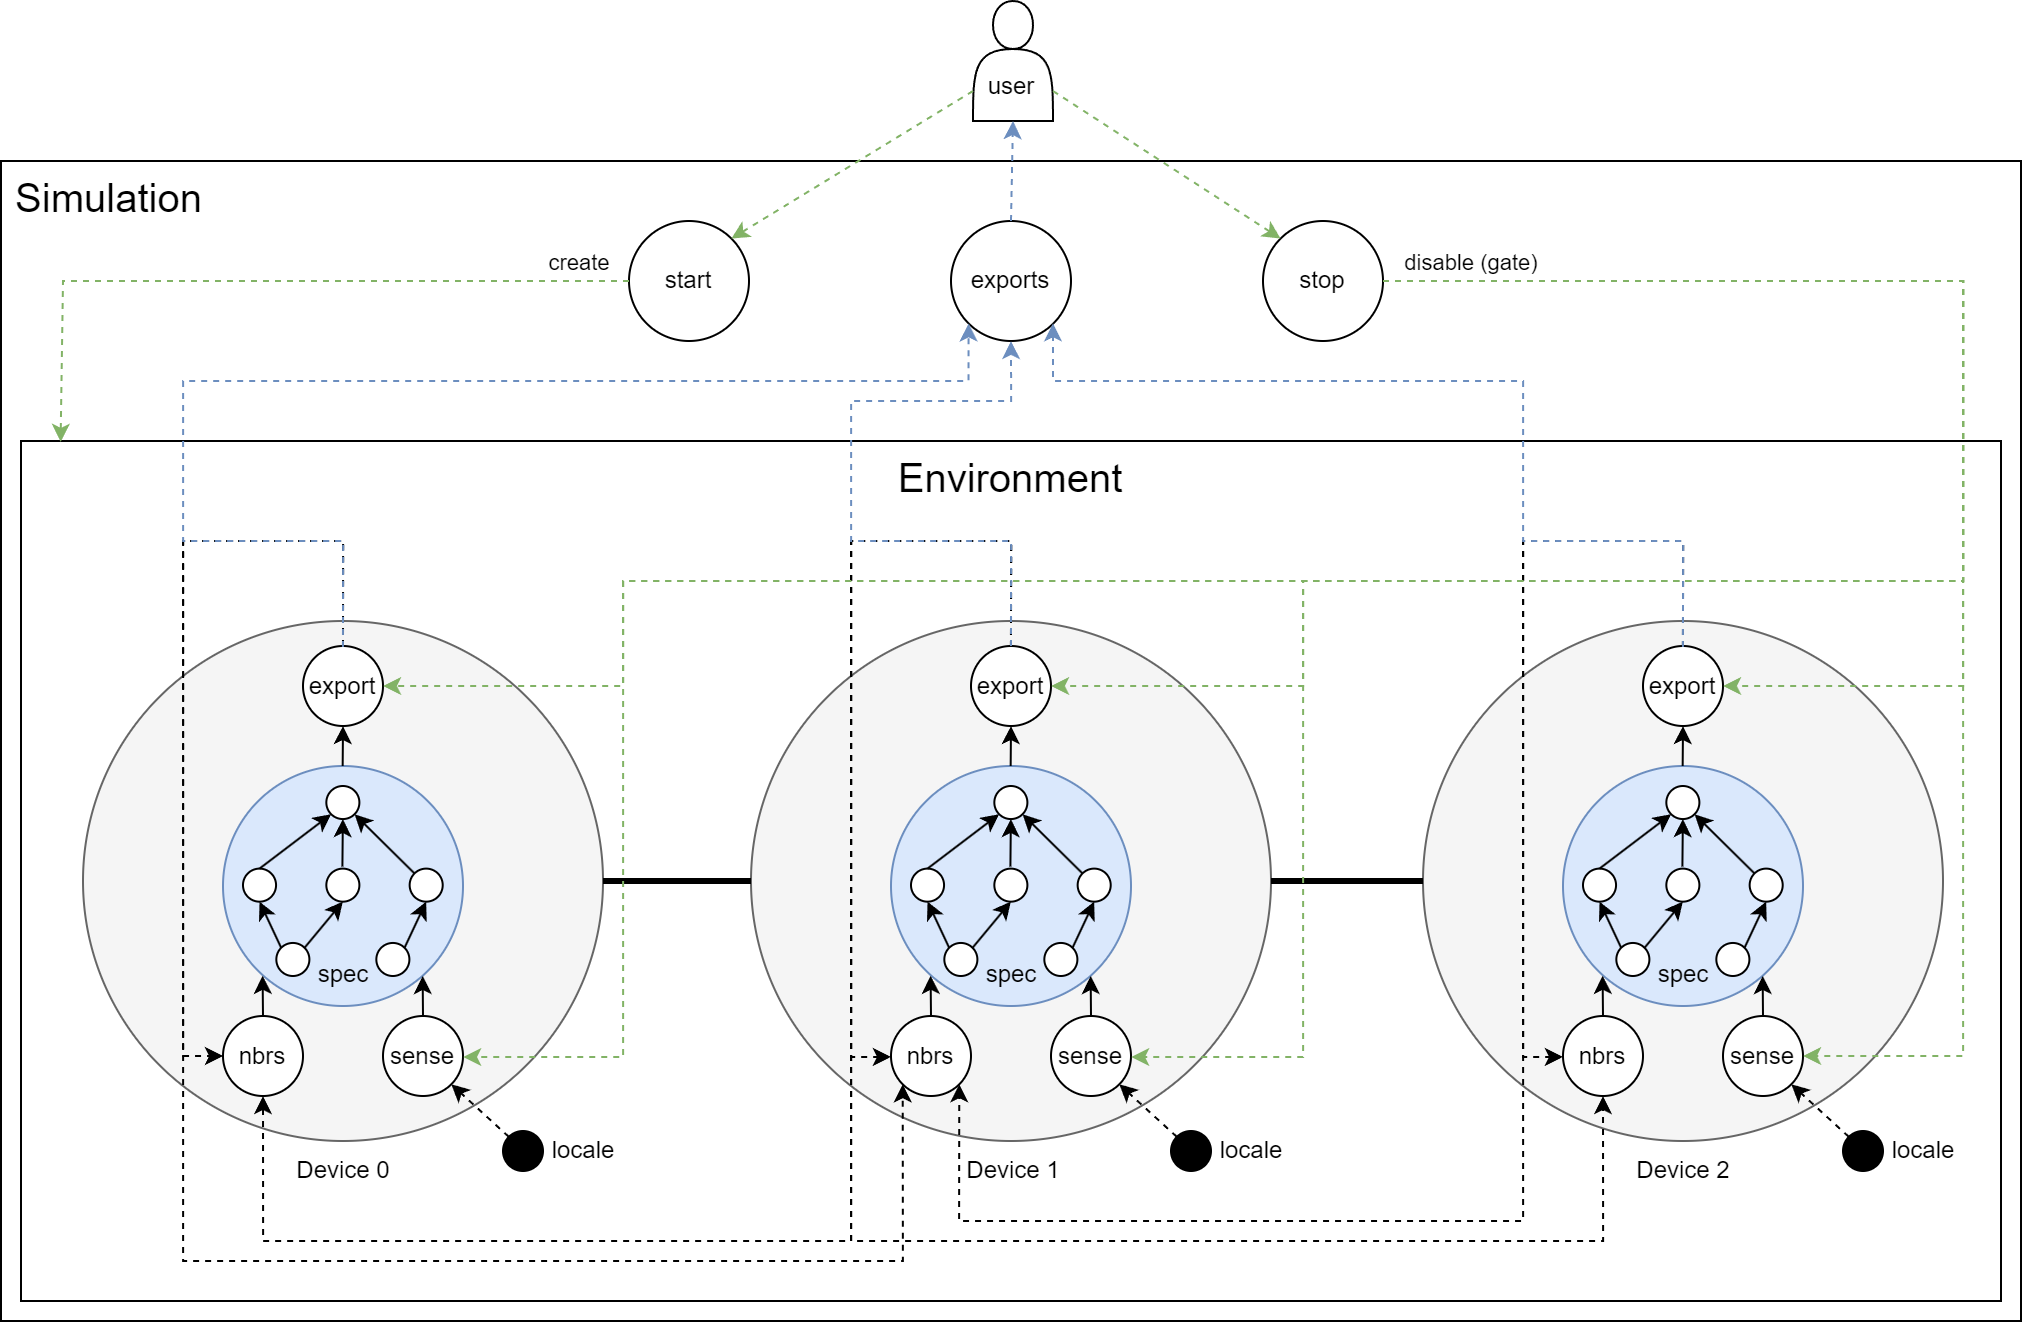
\includegraphics[width=1\textwidth]{resources/figures/simulation.png}
  \caption{
    The interface of a simulation for observing and controlling the
    underlying reactive execution model of FRASP. The user can now observe the
    state of a simulation (\texttt{exports}), start it (\texttt{start}) or stop
    it (\texttt{stop}). To support these new functionalities, new
    dependencies have been added for observability (\textit{blue dashed arrows})
    and controllability (\textit{green dashed arrows}).
  }
  \label{figure:simulation}
\end{figure}

Regarding observability, in static environments, the evolution of an aggregate
is uniquely described by its initial state and the sequence of device exports
(as discussed in Section \ref{section:analysis:aggregate-testing}). As a
consequence, complete observability of the evolution of an aggregate can be
achieved by simply collecting all the exports in the order they were produced,
whereas the initial state of the aggregate can be inferred from the
specification and environment provided during the configuration of the reactive
execution model (recall the configuration phase from Section
\ref{section:background:technologies:frasp}). In practice, the simulation
interface exposes a new reactive variable, called \texttt{exports}, derived by
\textit{merging} individual exports from each device. The firings of
\texttt{exports} can also be filtered, mapped and accumulated to provide
individual, regional or global views on the evolution of the aggregate.

Observability extends to dynamic environments by leveraging device sensors
(using the \texttt{sensor} and \texttt{nbrSensor} constructs) to reactively
produce exports containing changes in the environment.

Concerning controllability, the simulation interface offers a \texttt{start}
functionality, delaying the creation of the computational graph of the base
reactive execution model until requested by the user (instead of building the
graph when the simulation is created). This delay allows the user to declare
their own dependencies on the \texttt{exports} of the simulation before its
execution. As a consequence, forward referencing is required for
\texttt{exports} to declare its dependencies on the individual exports of the
devices.

To stop the simulation, it is possible to filter any future export when
requested by the user, freezing all views on the simulation (i.e.,
\texttt{exports}) and blocking any communication within the aggregate. However,
non-observable computation could still be triggered following a change in the
environment, even after the simulation is stopped. Therefore, to optimize the
simulation, any future percept of the device sensors should also be filtered
upon termination. Alternatively, the computational graph should be disposed of,
if possible.

An important aspect to consider for the observability of a simulation is
\textit{simulation time}, which measures the progress of a simulation. In
event-driven simulations, time is quantified as the number of events fired
since the beginning of the simulation (i.e., the number of firings of the
variable \texttt{exports}). Still, this representation has some implications,
such as time not advancing if no events are fired, affecting controllability.
Indeed, one cannot rely on the simulation time to stop the simulation without
prior knowledge about the evolution of the aggregate. For example, halting a
simulation after a specific number of events is unreliable, because one cannot
assume that the simulation will ever fire that many events, so the condition
may never be satisfied. However, a similar policy may be required to ensure
termination in aggregate tests, when the simulations never reach a stable
state, perhaps due to the nature of the specification or an unknown flaw in its
implementation.

Abstracting from the specific use case of halting the simulation, the problem
is that neither the user nor the simulation have an understanding of the
progress of the aggregate's evolution. On the one hand, the user lacks
information about the number of events that will be produced in the simulation,
which depends on the concrete implementations of the simulation and
specifications. On the other hand, the simulation lacks information about
possible changes of the environment, that may be triggered not only by the
device actuators, but also by external entities, such as the user. As a
consequence, none of the parties can evaluate when the evolution of the
aggregate should be considered concluded. This issue is referred to as the
\textbf{halting problem} in the following chapters.

% ! TeX root = ../../master-thesis.tex

\section{Step Simulation}
\label{section:design:step-simulation}

In order to address the halting problem, the previous simulation interface
should be refined to attain increased observability and controllability,
providing the user with more information about the state of the simulation. One
possibility is to model the concept of \textbf{step simulation}, which would
allow the user to execute a simulation step-by-step, receiving feedback after
every step (Figure \ref{figure:step-simulation}).

\begin{figure}[!ht]
  \centering
  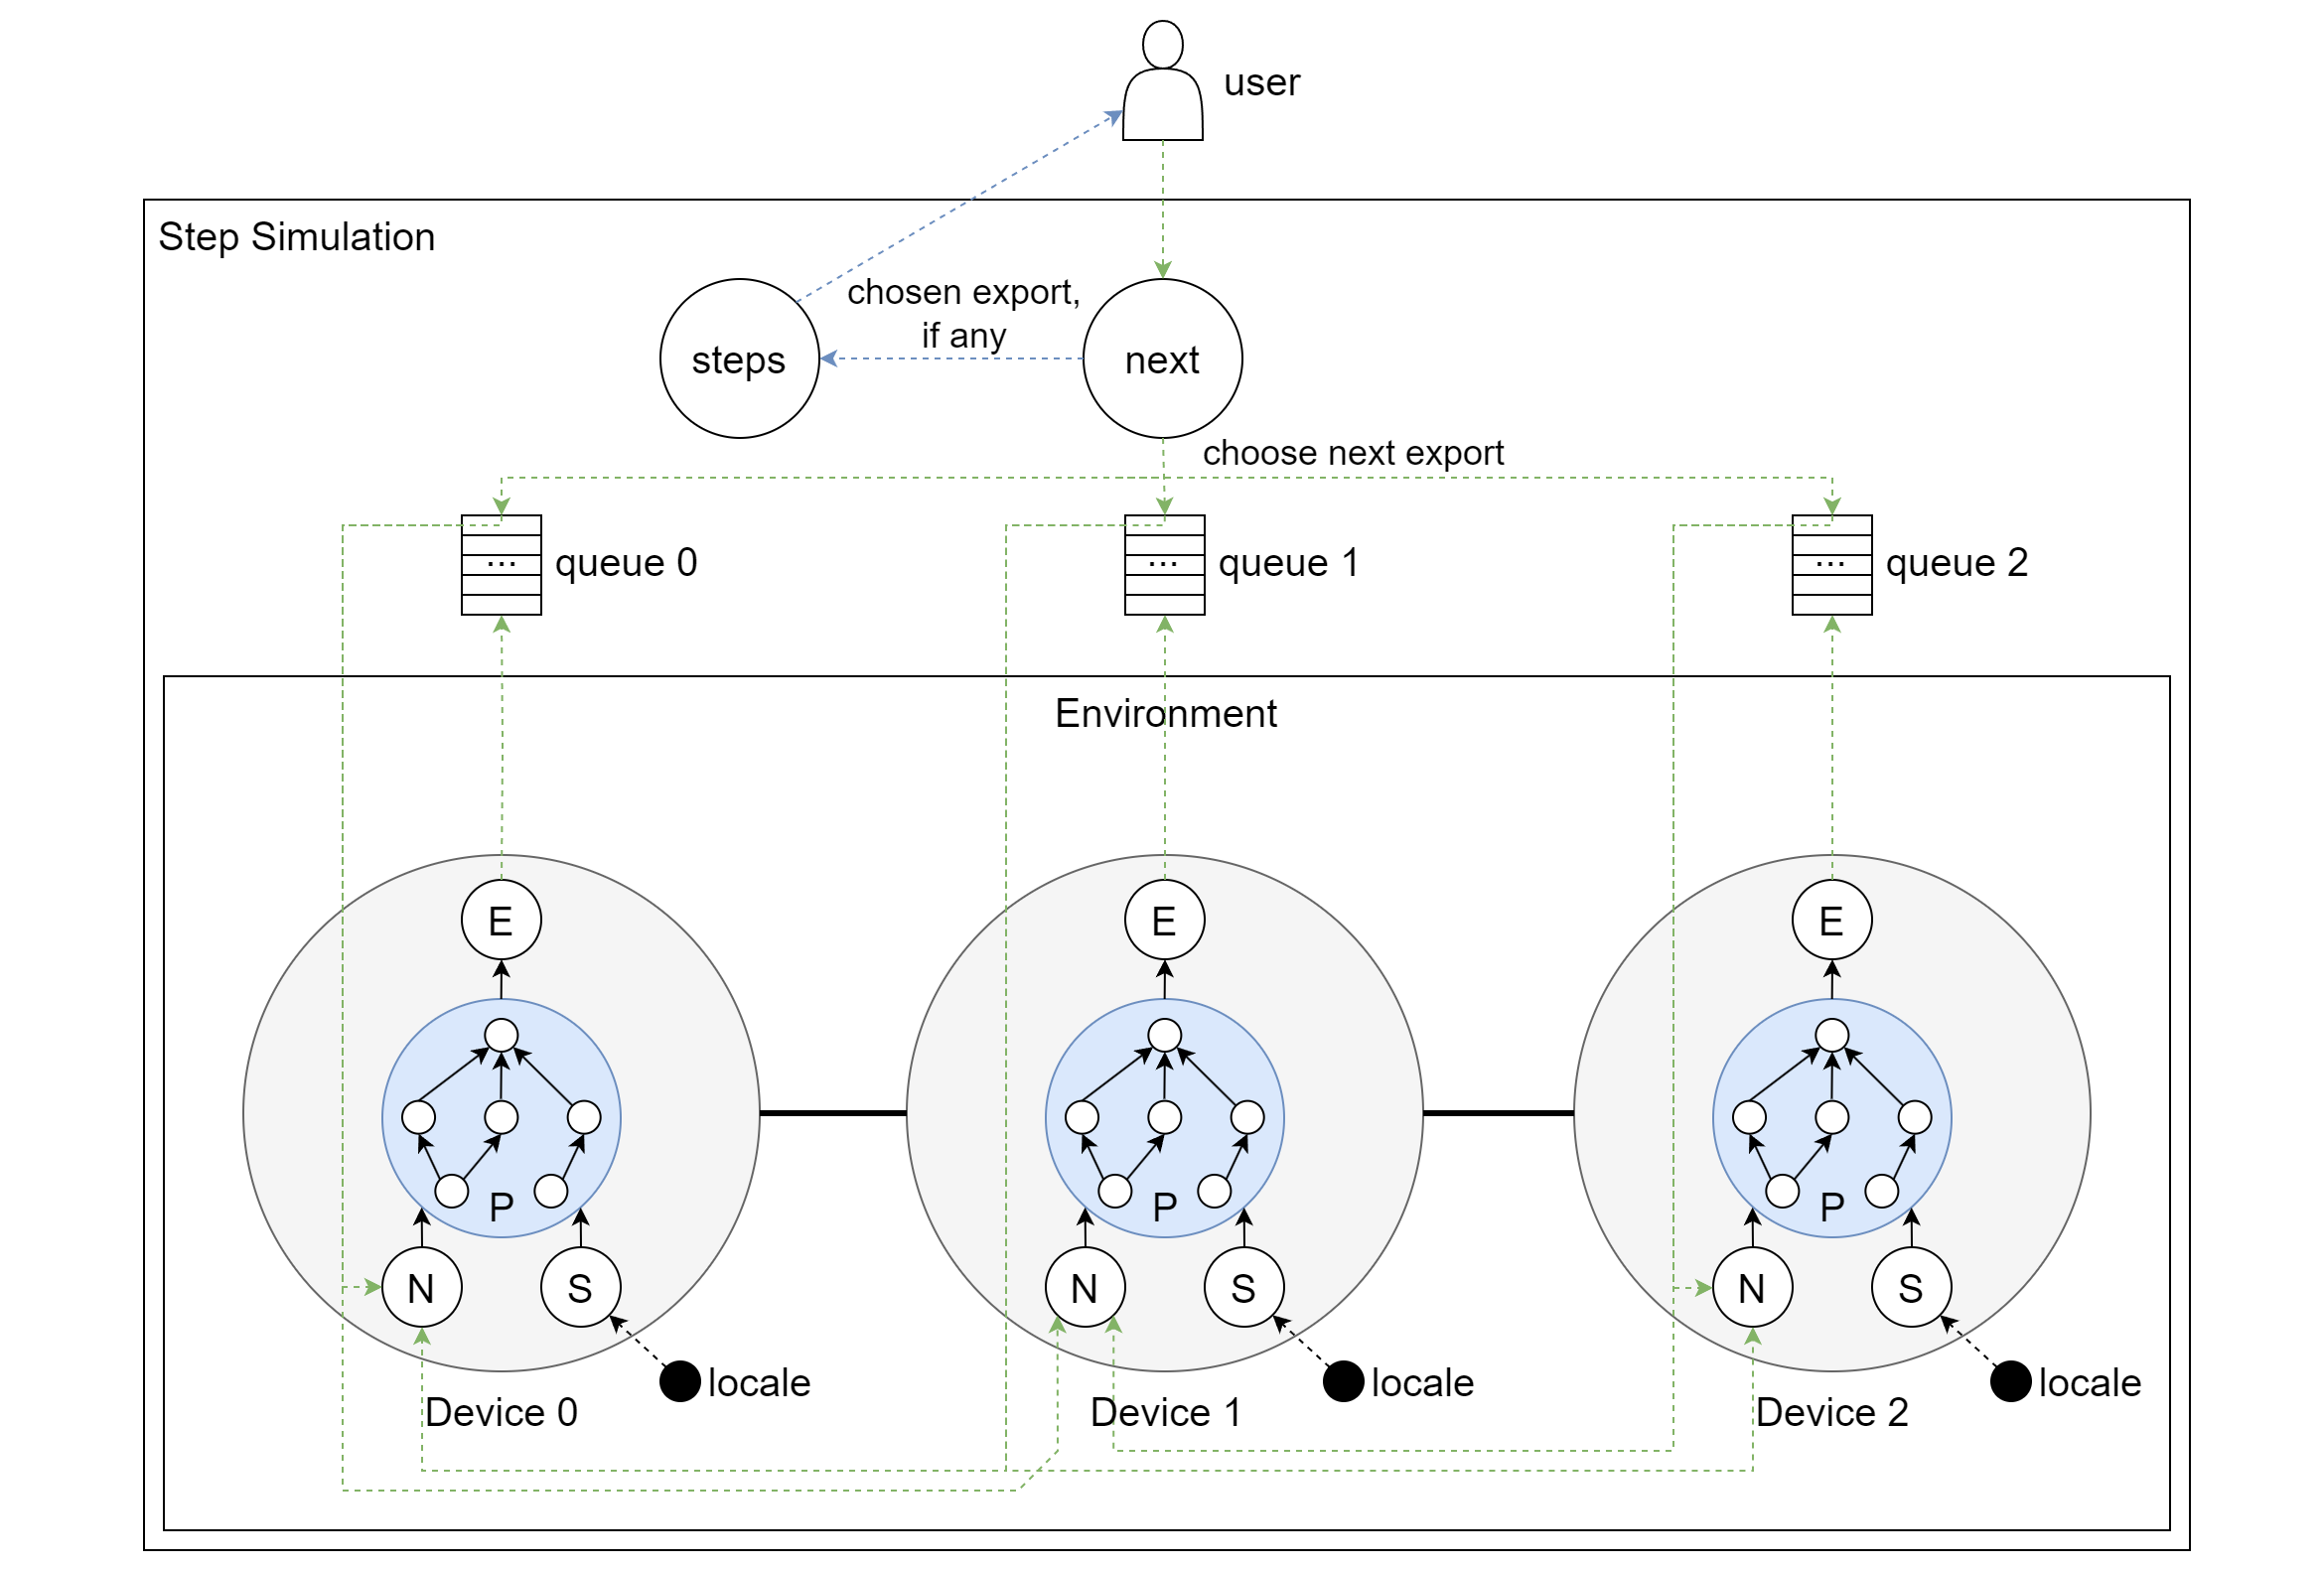
\includegraphics[width=1\textwidth]{resources/figures/step-simulation.png}
  \caption{The interface of a step simulation. Each device owns a queue of
    exports that need to be transmitted. In fact, when an export is produced, it
    is inserted in the queue of the corresponding device, instead of being
    broadcast directly to its neighbours. The interface exposes new
    functionalities for selecting, transmitting (\texttt{next}) and observing
    (\texttt{steps}) the next export from the queues, increasing observability
    (the user can be notified if there are no more exports to be transmitted)
    and controllability (the user can decide exactly when the simulation should
    continue). The other functionalities of simulations are supported, but
    hidden for clarity.}
  \label{figure:step-simulation}
\end{figure}

The concept behind a step simulation involves keeping track of the exports of
the devices, deferring their propagation until requested by the user. This
strategy achieves greater observability since the simulation knows precisely
the number of pending exports, allowing the user to be notified when there is
none. Controllability is also increased, as the user can decide exactly when
the simulation should continue. Ultimately, the halting problem is solved if
the user has complete control over the environment. Indeed, in this scenario,
the user can reasonably assume that the evolution of the aggregate has
concluded (and the simulation should be stopped) when there are no more exports
to propagate and no further intention to change the environment.

In detail, the simulation maintains a queue of exports for each device, so that
the device exports are pushed into the queue of the corresponding device when
produced. The user can request the execution of the next \textbf{step} (i.e.,
the propagation of the next export), then an export is extracted from one of
the device queues and transmitted to the neighbours. For each request, the user
is notified of the extracted export or the lack of pending exports through the
reactive variable \texttt{steps}. Note how the system behaves exactly like the
base reactive model of FRASP if a request is sent every time a new export is
produced.

An added benefit of this approach is the ability to manage the scheduling of
device exports. When a user request is received, the simulation takes charge of
selecting the next export to transmit. To this end, various scheduling policies
can be implemented. For instance, the next export can be extracted from one of
the non-empty queues chosen randomly, ensuring non-determinism in the
aggregate's evolution. Alternatively, a round-robin policy can be employed to
select the next export, ensuring fairness in the simulation.

Concurrency is also supported as events from different export queues may be
propagated at the same time. However, synchronization is required to guarantee
a consistent view of the simulation from the perspective of the user.

% ! TeX root = ../../master-thesis.tex

\section{Convergence Simulation}
\label{section:design:convergence-simulation}

The simulation interface can be extended once more to provide direct support
for aggregate convergence tests, exposing an operation for evaluating the limit
of an aggregate evolution with respect to time, that is a stable state for
self-stabilising specifications. To support such operation, during the
configuration phase, a simulation should accept a \textbf{halt policy}, which
is a condition that stops the simulation when satisfied. Moreover, such halt
policy should be designed so that the simulation is stopped when the aggregate
reaches a stable state.

For example, for a step simulation, a suitable halt policy would be to stop the
simulation when there are no more exports that can be extracted from the device
queues. Instead, for a general reactive simulation, a suitable halt policy
would be to stop the simulation after a certain period of inactivity (i.e.,
time elapsed since the last emitted event). However, real-world time introduces
non-determinism in the results of the simulations, rendering the policy not
suitable for testing.

% ! TeX root = ../../master-thesis.tex

\section{Concurrent Simulation}
\label{section:design:concurrent-simulation}

Concurrency in reactive simulations can be achieved by delegating the
propagation of change to some workers (e.g., a thread pool). In particular, in
Sodium, concurrency can be achieved by removing a dependency between a consumer
and a producer in a computational graph, then listening to the events of the
producer and delegating to a worker the propagation of each event towards the
consumer. However, this approach is limited to concurrency and cannot achieve
parallelism, due to Sodium's transactional system.

As discussed in Section \ref{section:background:technologies:sodium}, Sodium's
transactions are executed one at a time to guarantee glitch freedom, trading
off parallelism to ensure consistency. Later, it was discovered that
transactions are executed sequentially even among independent computational
graphs. Therefore, unless the computation of a device is detached from the
computational graph (i.e., executed outside the FRP engine), concurrent
simulations cannot be executed in parallel, in fact concurrent events are still
processed sequentially.

Moreover, the deployment of the reactive execution model in real distributed
systems is still unclear, possibly hinting towards the research of distributed
reactive programming solutions. Further research could discover the effects of
Sodium's consistency in the evolution of aggregate of devices and evaluating
the possibility of achieving the same level of consistency in large-scale
distributed systems, such as \ac{CAS}s.
